\wip
\section{Hardware-Konfiguration}
Die aktuelle Hardware der Station setzt sich aus mehreren Einzel-Platinen mit unterschiedlichen Betriebsspannungen zusammen:
\begin{itemize}
    \item Mikrofon-Vorverstärker-Platine, die das Signal des Kondensator-Mikrofons verstärkt, bevor es zum \ac{rpi} weitergeleitet wird. Diese Platine wird mit einer Spannung von 5VDC betrieben.
    \item Lautsprecher-Verstärker-Platine, die für die Verstärkung der wiederzugebenden Audiosignale des \ac{rpi} zuständig ist. Die verstärkten Signale werden direkt an den Lautsprecher der Station übergeben. Diese Platine benötigt eine Versorgungsspannung von 24VDC.
\end{itemize}
Die elektrische Versorgung der Station erfolgt mittels \ac{poe} bei einer Speisespannung von etwa 30VDC.
Alle Platinen sind mit Heißkleber in der Station montiert.

\section{Problemdefinition}
\paragraph{Systemstabilität:} %poe
In der aktuellen Konfiguration kommt es immer wieder zu unvorhersehbaren und unkontrollierten Systemabstürzen.
Die betroffene Station reagiert weder auf eingehende Signale, noch erfolgt irgendeine Form der Informationsausgabe.
Dieser Zustand lässt sich nur durch ein Zurücksetzen des Prozessors beenden.
Die Abstürze sind bei der am weitesten von der Spannungsversorgung entfernten Station am häufigsten zu beobachten.
Dieser Fehler tritt in unregelmäßigen Abständen von bis zu mehreren Monaten auf.
Die betroffene Station weist keinen Hardware-Unterschied zu den anderen Stationen auf.
Daher lässt sich vermuten, dass die Länge und Art der Verkabelung mit diesem Phänomen in Zusammenhang steht.

\paragraph{Komplexer Aufbau:} %einzelplatinen
Die aktuelle Hardware-Konfiguration verwendet einige Einzelplatinen, die miteinander über eine fliegende Verdrahtung verbunden sind.
Dies reduziert die Übersichtlichkeit des Stationsinneren und birgt die Gefahr von fehlerhafter Verdrahtung in sich.
Durch die fliegende Verdrahtung ist kein einheitliches Erscheinungsbild des Stationsinneren gewährleistet.

\paragraph{Brumm-Schleife:} %gnd-loop
Die aktuelle Verdrahtung führt zu einer Masseschleife.
Diese erzeugt ein konstantes Störgeräusch.
Über die Verstärkerschaltung führt dies zu einem unerträglichen Brumm-Ton.
In der aktuellen Hardware-Konfiguration wird das Problem mit einer Massetrennung nach dem Ausgang des \ac{rpi} umgangen.
Dieser zusätzliche Baustein wurde fliegend verdrahtet und mit Heißkleber befestigt.

Folgend ein Bild der aktuellen Station und deren Verdrahtung.
\begin{figure}[H]
    \centering
    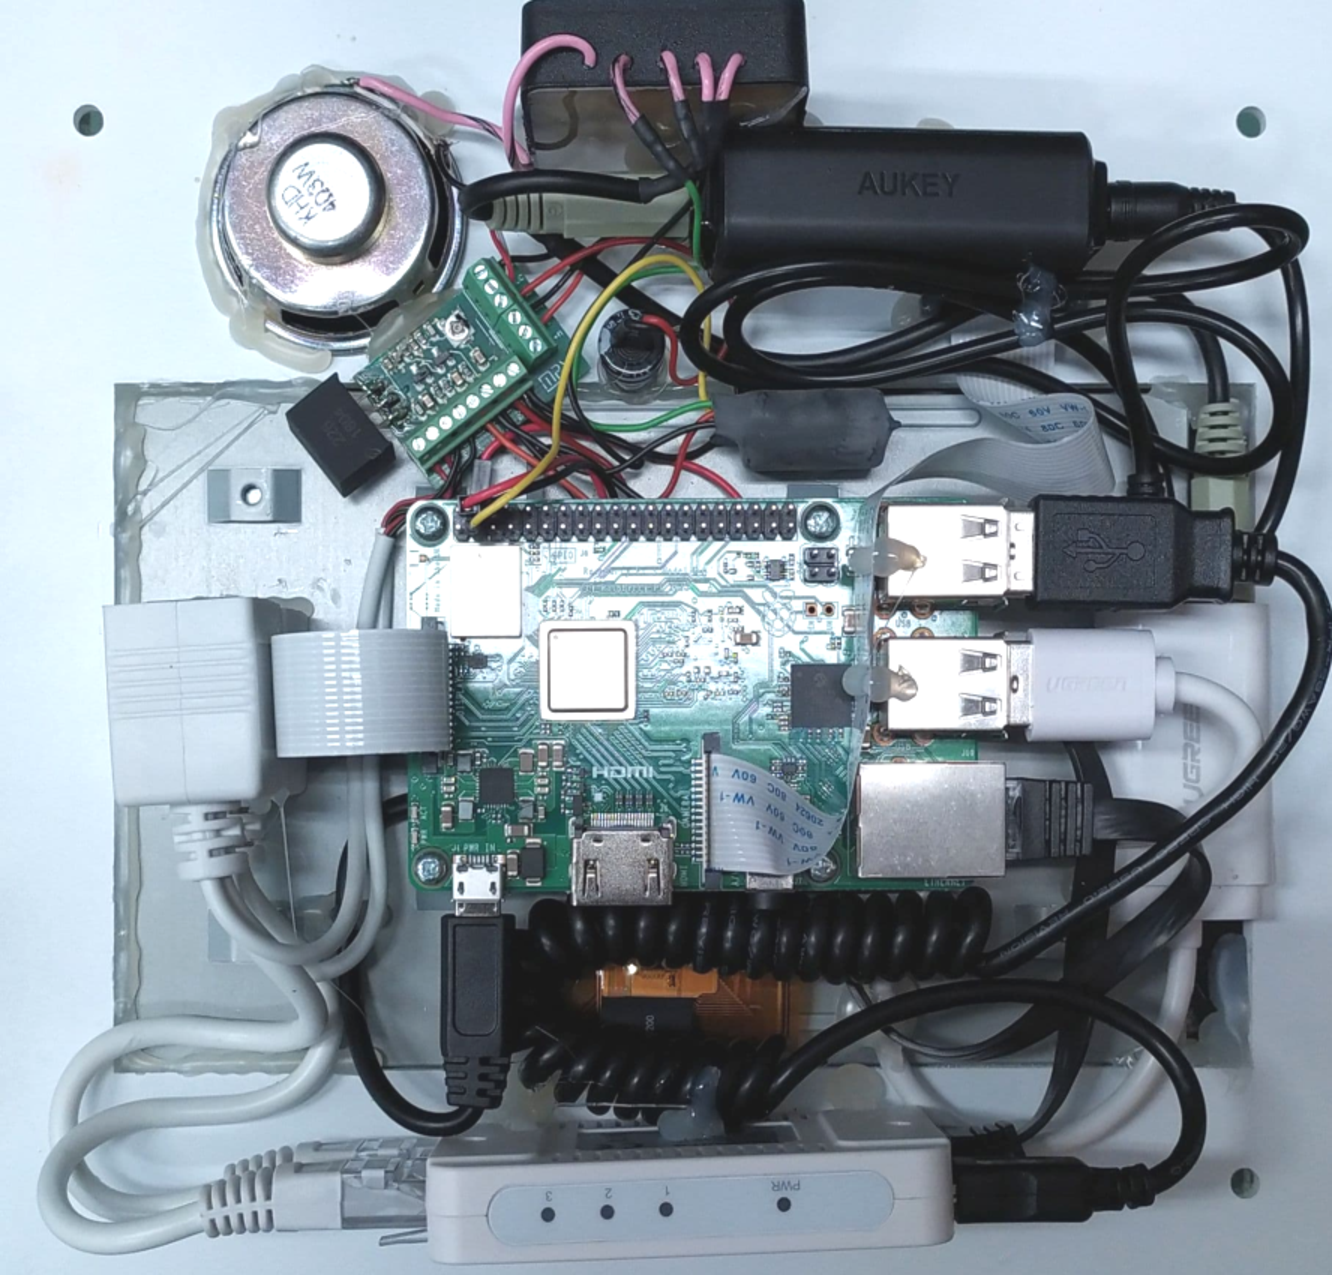
\includegraphics[width=.9\linewidth]{images/ist_situation/fliegender_aufbau.pdf}
    \caption{Unübersichtliche Verdrahtung}
\end{figure}